\documentclass{article}
\usepackage{amsmath}
\usepackage{graphicx}
\usepackage{siunitx}
\usepackage{float}
\usepackage{gensymb}
\usepackage[dvipsnames]{xcolor}
\usepackage{sectsty}

%\setlength{\parskip}{1em}

%\definecolor{color:background}{RGB}{40,40,40}
%\definecolor{color:text}{RGB}{230,230,230}

%\pagecolor{color:background}
%\color{color:text}
%\allsectionsfont{\normalfont\sffamily\bfseries}

\title{ELEC344 Assignment 2}
\author{Kelvin Hsu}


\begin{document}
    \sffamily
   	\maketitle
    \newpage

\section*{1)}
    \begin{figure}[H]
        \centering
        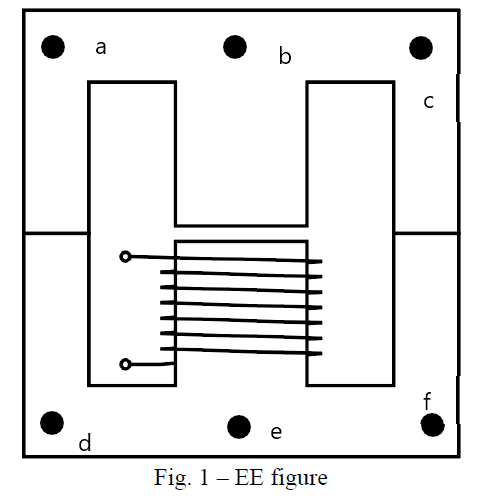
\includegraphics[width=10cm]{figures/e-mag.PNG}
        \label{fig:e_mag}
    \end{figure}


    \subsection*{a.}
    \begin{align*}
        &R_{air} = \frac{l}{\mu A} = \frac{10^{-3}}{7.5*10^{-3}*7.5*10^{-3}*4\pi *10^{-7}} = 1414710.605\\
        &R_{be core} = \frac{l}{\mu A} = \frac{2* 10.25 *10^{-3}}{7.5*10^{-3}*7.5*10^{-3}*4\pi *10^{-7} * 1620} = 179.022\\
        &R_{ac} = \frac{l}{\mu A} = \frac{21.25* 10^{-3}}{7.5*10^{-3}*4.1*10^{-3}*4\pi *10^{-7} * 1620} = 186881.5244\\
        &R_{af} = \frac{l}{\mu A} = \frac{21.5 *10^{-3}}{3.75*10^{-3}*7.5*10^{-3}*4\pi *10^{-7} * 1620} = 186881.5244
    \end{align*}
    
    \begin{align*}
        R_{total} &= R_{air} + R_{be_core}  + [(R_{ac}+R_{af})||(R_{ac}+R_{af})]\\
        &= R_{air} + R_{be_core}  + \frac{(R_{ac}+R_{af})}{2}\\
        &= \boxed{14683613 (AT/W)}\\
        A_{L} &= \frac{1}{R_{total}} = 6.8*10^{-8}
    \end{align*}
    \subsection*{b.}
    \begin{align*}
        Li = N \Phi\\
        L = 0.00004256H
    \end{align*}
    
    \subsection*{c.}
    \begin{align*}
        L = \frac{N \Phi}{i}\\
        B = 390 mT\\
        i = \frac{NBA}{L} = 12.89A
    \end{align*}
    
    \subsection*{d.}
    When current exceeds the maximum current, the core is saturated and 
    the reluctance increases.(the slope of B-H graph decrease to $\mu_{air}$). 
    Consequently, the inductance decreases since $L = \frac{N^{2}}{R}$.
        
    \section*{3}
    \subsection*{a.}
    \begin{align*}
        &V_{a} = e_{a}  + i_{a}R_{a} + L_{a}\frac{di_{a}}{dt}\\
        &T_{e} = J_{L} \frac{d\omega_{m}}{dt} + B_{L}\omega + T_{L}\\
        &\frac{d\omega_{m}}{dt} = 0\\
        &\frac{di_a}{dt} = 0\\
        &V_{a} = e_{a} + i_{a}R_{a}\\
        &i_{a} = \frac{T_{e}}{k_{T}}\\
        &e_{a} = k_{e}\omega_{m}\\
    \end{align*}

    \begin{equation*}
        \boxed{T_{e} = \frac{k_{T}}{R_{a}}[V_{a} - k_{e}\omega]}
    \end{equation*}

    \begin{figure}[H]
        \centering
        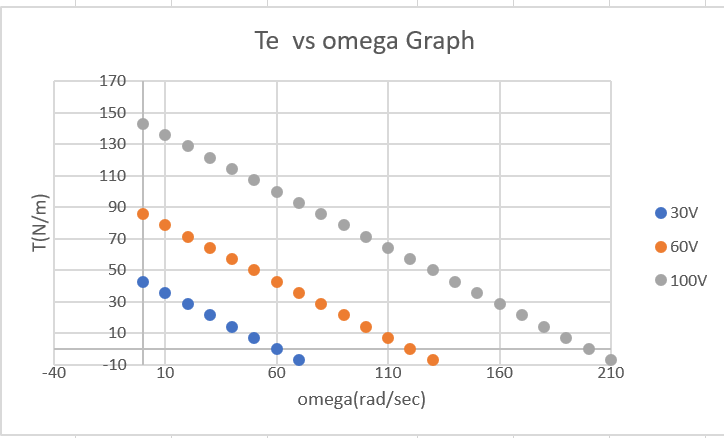
\includegraphics[width=10cm]{figures/t_omega.PNG}
        \label{fig:t_omega}
    \end{figure}
    \subsection*{b.}
    \begin{align*}
        V_{a} &= 0.5\frac{V}{rad*s}*157rad/s + \frac{3 Nm}{0.5 Nm/A}*0.35\ohm\\
        &= 80.6V
    \end{align*}

    \section*{4}
    \subsection*{a)}
    \begin{align*}
        &Z_{1} = (j X_{m}) || (\frac{R_{2}}{s} + j X_{e2})\\
        &Z_{1} = 2.47 \angle 18.98\\
        &Z_{total} = R_{1} + jX_{e} + Z_{1} = 2.84\angle 25.76\\
        &i_{stator} = \frac{V_{source}}{Z_{total}} = \boxed{42.24\angle -25.76}
    \end{align*}

    \begin{equation*}
        P_{copper} = 3 * I_{stator}^{2} * R_{1} = \boxed{1178W}
    \end{equation*}

    \subsection*{b)}
    \begin{align*}
        &P_{ag} = E_{ag} \cdot I_{rotor} \cdot 3 = 3 * I_{stator}^{2} * Z_{1} = \boxed{12500W}\\
        &\frac{P_{em}}{P_{ag}} = (1-s)s = 0.95\\
        &\boxed{P_{em} = 11880W}
    \end{align*}

    \subsection*{c)}
        \begin{equation*}
            P_{rotor_loss} = P_{ag} - P_{em} = \boxed{620W}
        \end{equation*}
    
        \begin{align*}
            \omega_{synchronous} = \frac{2}{p} * 2\pi f = 288.49 rad/s\\
            T_{em} = \frac{P_{em}}{\omega_{synchronous}} = \boxed{66.3Nm}
        \end{align*}

        \begin{align*}
            P_{out} = 3\cdot 120 \cdot 42.25 cos(-25.76) - 1178 - 0.2k - 0.62k - 0.3k = 11.4k\\
            T_{L} = \frac{P_{out}}{\omega_{m}} = \frac{P_{out}}{(1-s)\omega_{synchronous}} = 63.7 3Nm
        \end{align*}
    
    \subsection*{d)}
        \begin{equation*}
            \frac{P_{out}}{P_{in}} = 83.2\% 
        \end{equation*}


    \subsection*{e)}
        \begin{equation*}
            \omega_{m} = (1-s)\omega_{synchronous} = 179rad/s = 1709 RPM
        \end{equation*}

\end{document}